\pagestyle{n-1}
\label{n-1}

\begin{textblock*}{5.625in}(0pt,0pt)%
\vspace*{-1.45cm}
\hspace*{-1.8cm}\includegraphics*[width=112mm]{./imgs/N-1.png}
\end{textblock*}

\pagebreak

\hspace{.5cm}

\begin{center}
\hspace*{-1cm}\raisebox{5.5cm}{\rotatebox[origin=t]{90}{\Formular{\textbf{Lançamento}}}}
\hspace*{1cm}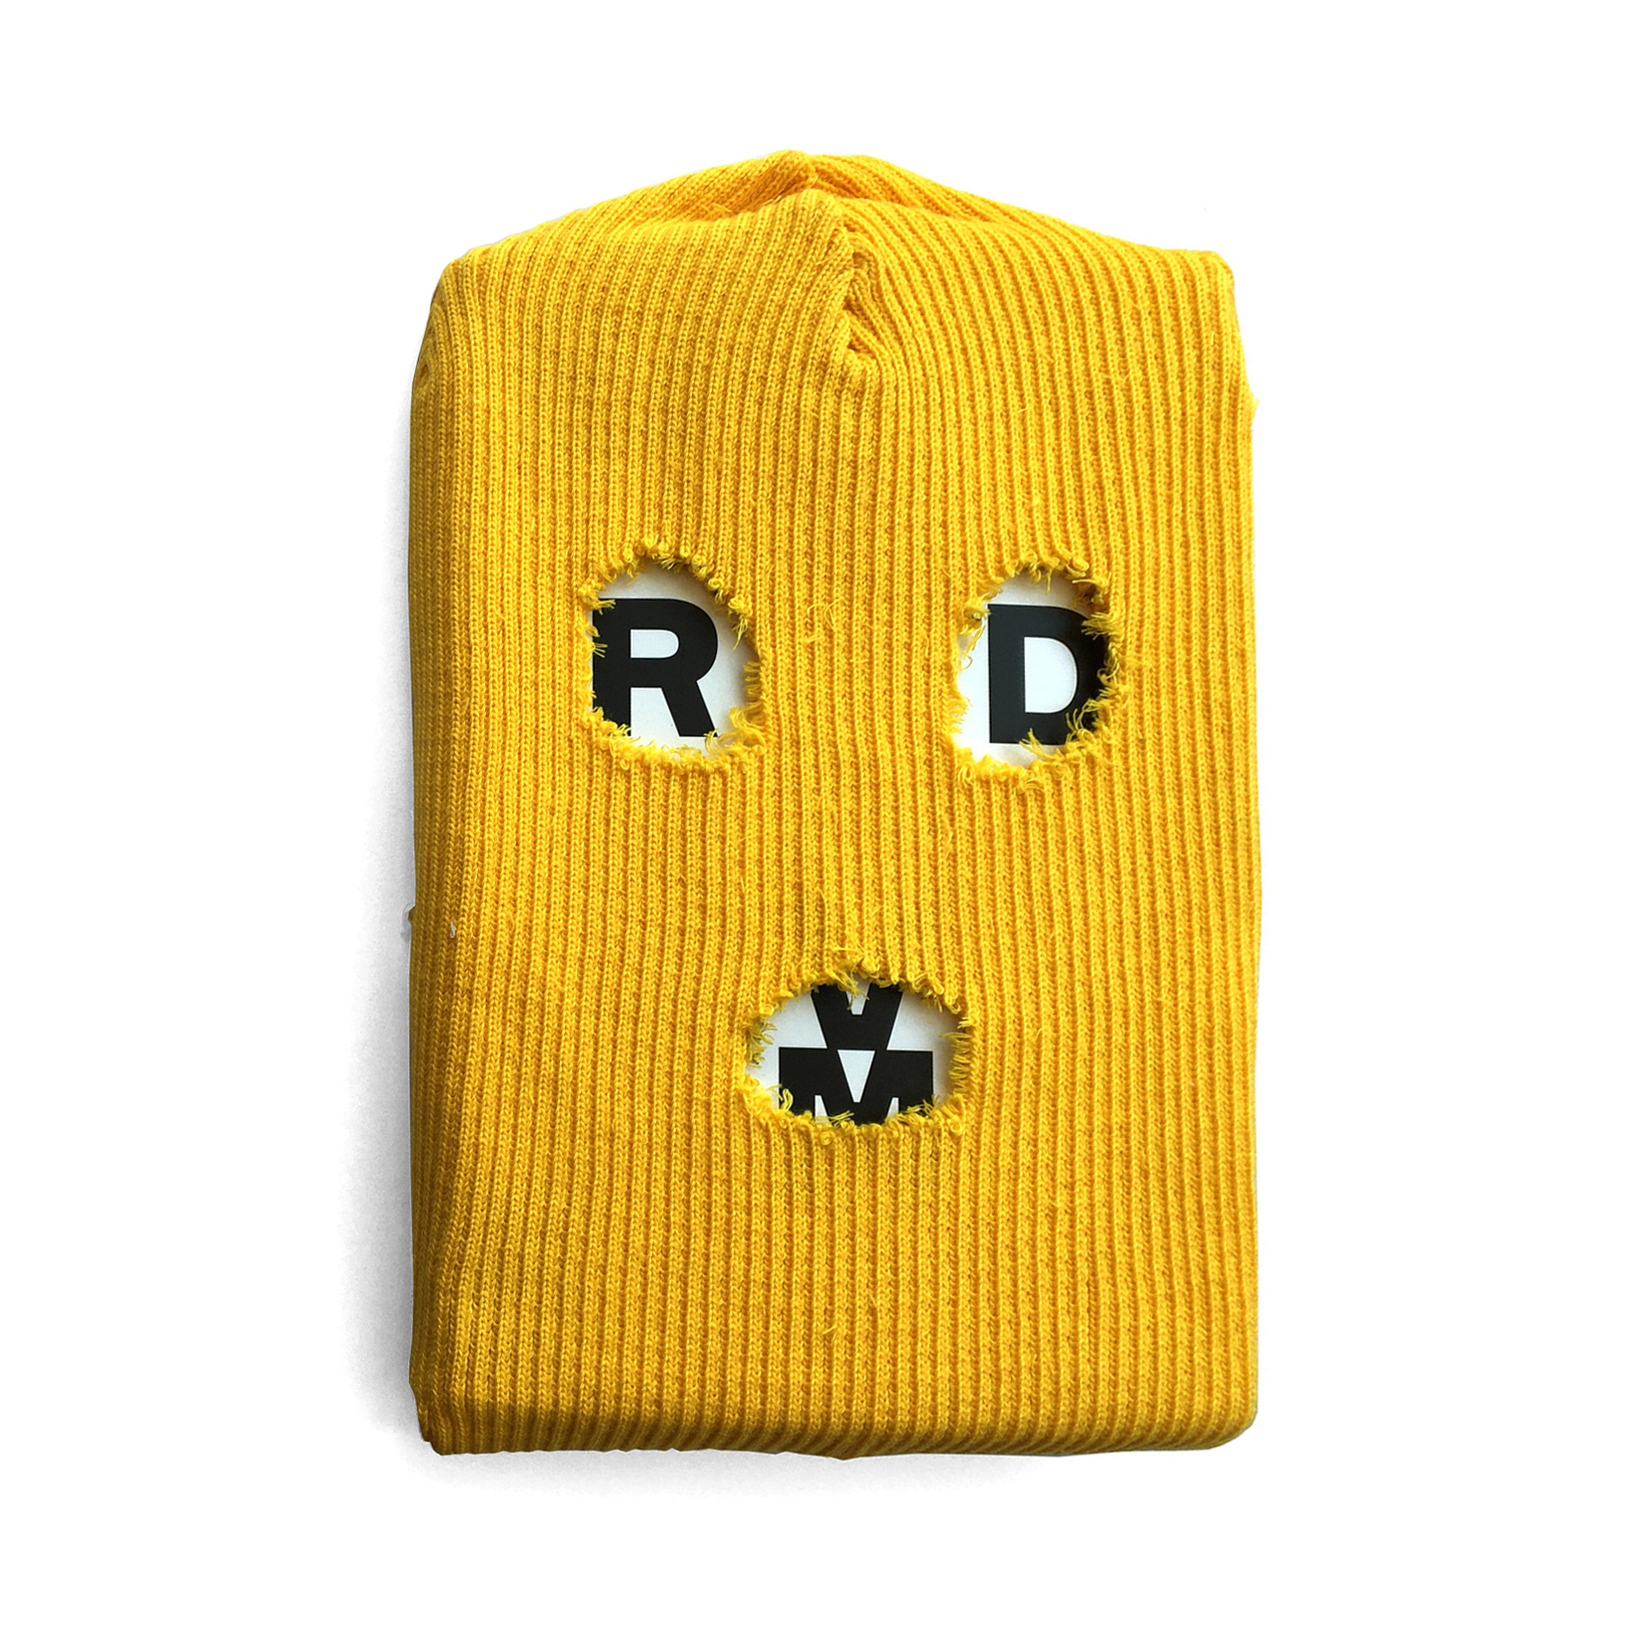
\includegraphics[width=70mm]{./grid/riot.jpg}
\end{center}

\hspace*{-7cm}\hrulefill\hspace*{-7cm}

\medskip

\noindent{}{\slsc{Riot Days}} é um relato cru, alucinatório e apaixonado sobre a prisão e julgamento da autora, Maria Alyokhina, em uma colônia penal após participar de um protesto punk contra Putin em uma igreja ortodoxa. Com tradução de Marina Damaros, os livros virão acompanhados por dois cordéis e serão embalados em balaclavas coloridas confeccionadas especialmente pela Cooperativa Libertas, de mulheres egressas do sistema penitenciário brasileiro.

\vfill

\hspace*{-.4cm}\begin{minipage}[c]{1\linewidth}
\small{
{\Formular{\textbf{
\hspace*{-.1cm}Título: Riot Days\\
Autor: Maria Alyokhina\\ 
Editora: n-1 / Hedra\\
Páginas: 216\\
Formato: 14x21cm\\
Preço: R\$ 89,90\\
ISBN: 978-65-8109-713-4
}}}}
\end{minipage}

\pagebreak

\hspace{.5cm}

\begin{center}
\hspace*{-.5cm}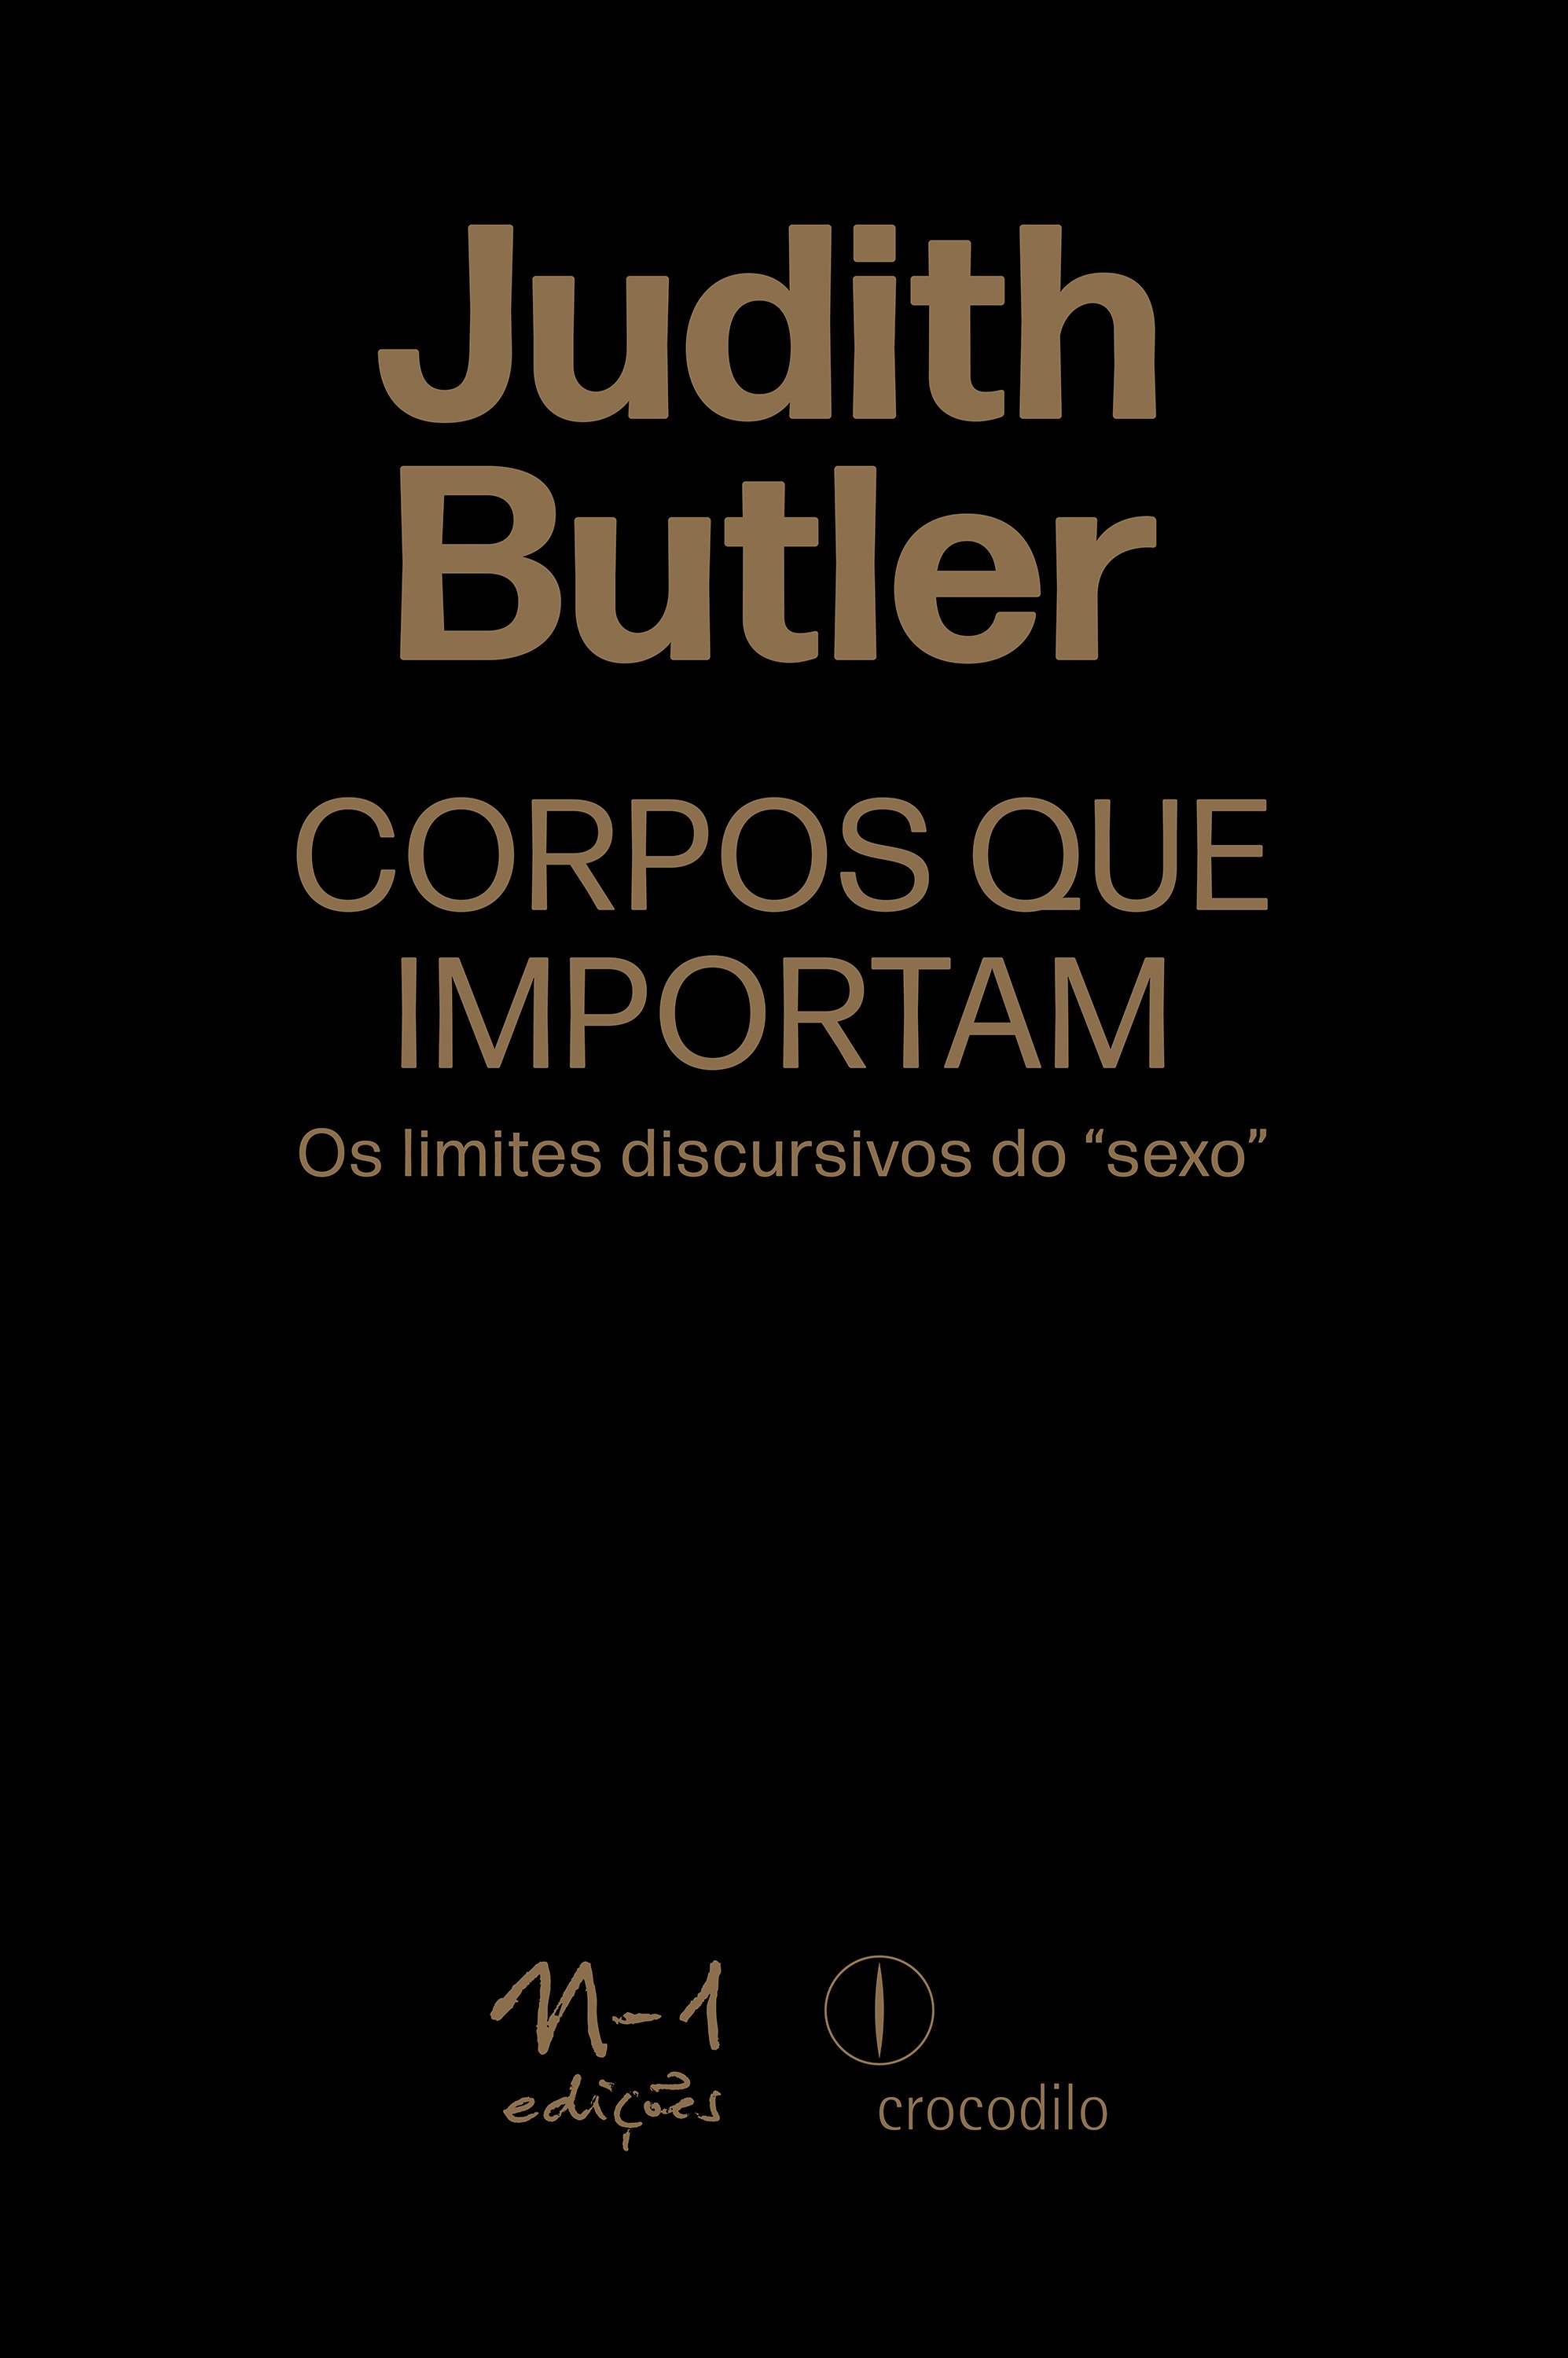
\includegraphics[width=46.6mm]{./imgs/butler.jpg}
\end{center}

\hspace*{-7cm}\hrulefill\hspace*{-7cm}

\medskip

\noindent{}{\slsc{Corpos que importam}} é um esforço para pensar mais sobre o funcionamento da hegemonia heterossexual na criação de matérias [{\slsc{matters}}] sexuais e políticas. Quais são as limitações pelas quais os corpos são materializados como “sexuados” e como devemos entender a “questão” [{\slsc{matter}}] do sexo, e dos corpos de modo mais geral, como a circunscrição repetida e violenta da inteligibilidade cultural? Quais corpos importarão [{\slsc{matter}}] – e por quê?

\vfill

\hspace*{-.4cm}\begin{minipage}[c]{1\linewidth}
\small{
{\Formular{\textbf{
\hspace*{-.1cm}Título: Corpos que importam – os limites discursivos do “sexo”\\
Autor: Judith Butler\\ 
Editora: n-1 / Crocodilo\\
Páginas: 400\\
Formato: 14x21cm\\
Preço: R\$ 98,00\\
ISBN: 978-65-8109-704-2
}}}}
\end{minipage}

\pagebreak

\hspace{.5cm}

\begin{center}
\hspace*{-2.5cm}\raisebox{5.5cm}{\rotatebox[origin=t]{90}{\Formular{\textbf{Lançamento}}}}
\hspace*{2cm}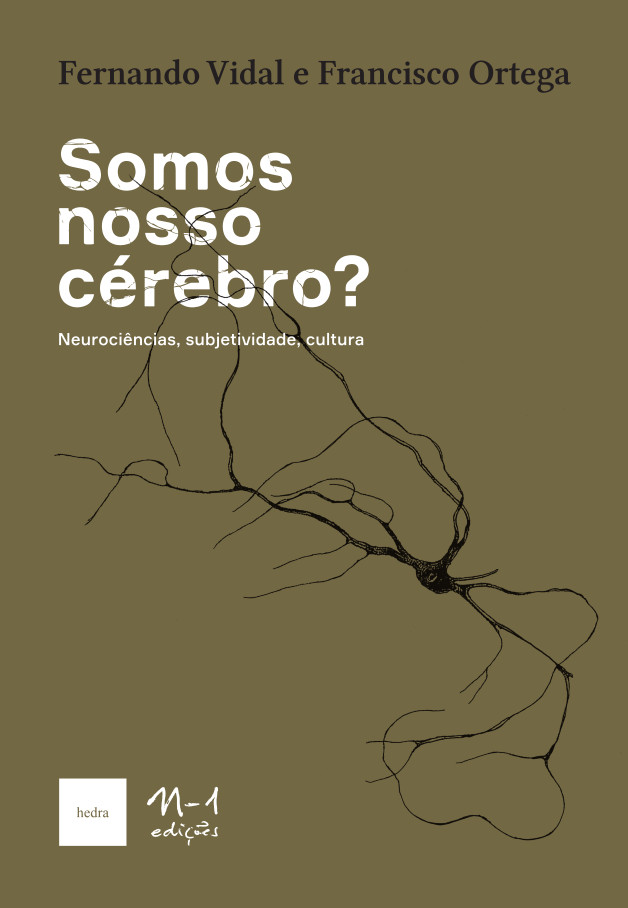
\includegraphics[width=45mm]{./imgs/cerebro.jpeg}
\end{center}

\hspace*{-7cm}\hrulefill\hspace*{-7cm}

\medskip

\noindent{}{\slsc{Somos nosso cérebro?}}, escolhido livro do ano em 2018 pela {\slsc{International Society for the History of the Neurosciences}}, oferece uma exploração crítica do neurocentrismo, a crença de que “somos nossos cérebros”, que está no cerne de alguns dos mais importantes debates da atualidade. Para tanto, examina a lógica interna de tal ideologia, sua genealogia e as suas múltiplas encarnações contemporâneas.

\vfill

\hspace*{-.4cm}\begin{minipage}[c]{1\linewidth}
\small{
{\Formular{\textbf{
\hspace*{-.1cm}Título: Somos nosso cérebro? Neurociências, subjetividade, cultura\\
Autor: Francisco Ortega e Fernando vidal\\ 
Editora: n-1 / Hedra\\
Páginas: 346\\
Formato: 16x23cm\\
Preço: R\$ 80,00\\
ISBN: 978-65-9582-035-7
}}}}
\end{minipage}

\pagebreak

\hspace{.5cm}

\begin{center}
\hspace*{-.5cm}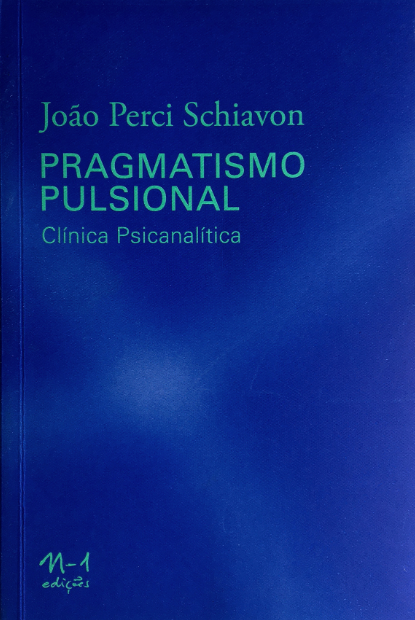
\includegraphics[width=45.8mm]{./imgs/gozo.png}
\end{center}

\hspace*{-7cm}\hrulefill\hspace*{-7cm}

\medskip

\noindent{}O saber ou o gozo pulsional tem esse traço de não servir a nenhum bem, algo meio desconcertante se tivermos em vista o título deste escrito: “pragmatismo pulsional”. A pulsão é o não sujeitável, a {\slsc{phisis}} freudiana, indicando a presença do originário no homem e no pensamento, uma autoridade no que diz respeito ao vivo ou ao desejo. Ela só precisa ser exercida. Cura é o nome que damos a esse exercício.

\vfill

\hspace*{-.4cm}\begin{minipage}[c]{1\linewidth}
\small{
{\Formular{\textbf{
\hspace*{-.1cm}Título: Pragmatismo pulsional – clínica psicanalítica\\
Autor: João Perci Schiavon\\ 
Editora: n-1\\
Páginas: 336\\
Formato: 14x21cm\\
Preço: R\$ 66,00\\
ISBN: 978-65-8109-706-6
}}}}
\end{minipage}

\pagebreak

\hspace{.5cm}

\begin{center}
\hspace*{-2.5cm}\raisebox{5.5cm}{\rotatebox[origin=t]{90}{\Formular{\textbf{Lançamento}}}}
\hspace*{2cm}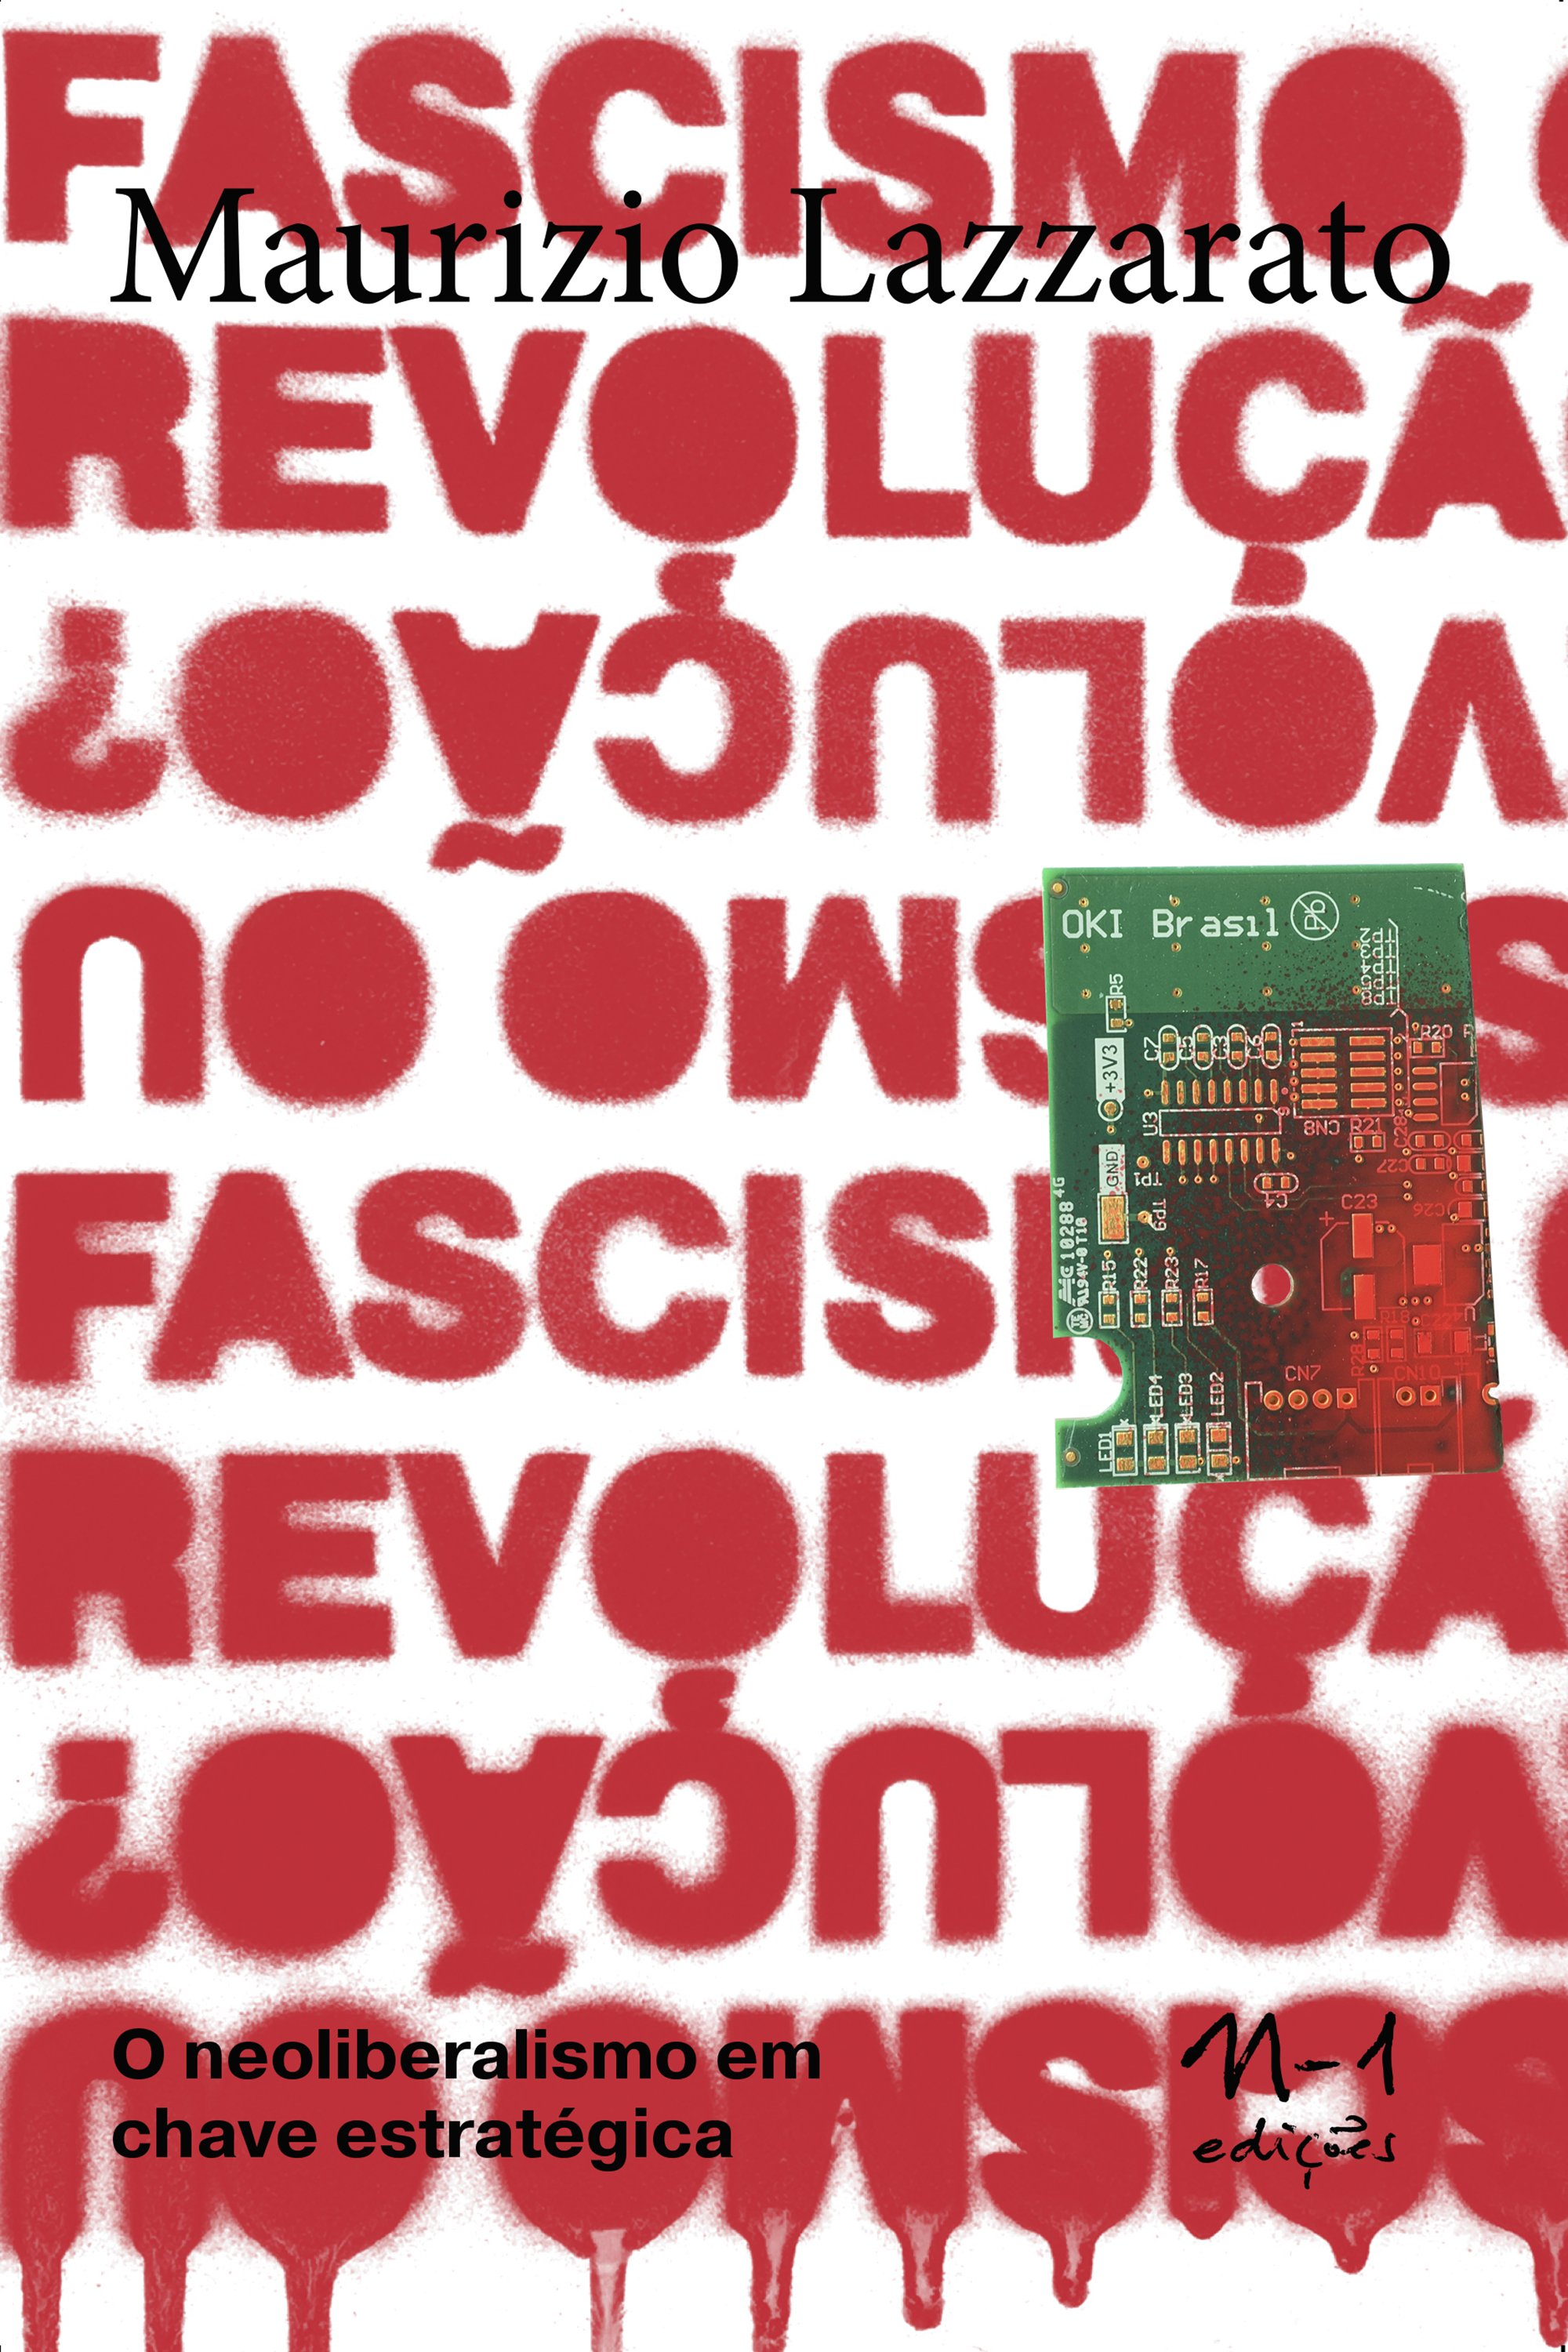
\includegraphics[width=45mm]{./imgs/lazzarato.jpg}
\end{center}

\hspace*{-7cm}\hrulefill\hspace*{-7cm}

\medskip

\noindent{}{O fascismo histórico foi tão moderno quanto o capitalismo, e também o é o novo fascismo, que é um ciberfascismo. Ele põe em xeque todas as utopias que viam nas máquinas cibernéticas a promessa de uma nova subjetividade pós"-humana livre do capitalismo. Bolsonaro e Trump se utilizaram da comunicação digital: são o resultado de uma máquina política que agencia uma micropolítica dos afetos tristes com a macropolítica de um novo fascismo.

\vfill

\hspace*{-.4cm}\begin{minipage}[c]{1\linewidth}
\small{
{\Formular{\textbf{
\hspace*{-.1cm}Título: Fascimo ou Revolução?\\
Autor: Mauricio Lazzarato\\ 
Editora: n-1\\
Páginas: 208\\
Formato: 14x21cm\\
Preço: R\$ 69,00\\
ISBN: 978-85-6694-381-8 
}}}}
\end{minipage}

\pagebreak

\hspace{.5cm}

\begin{center}
\hspace*{-.5cm}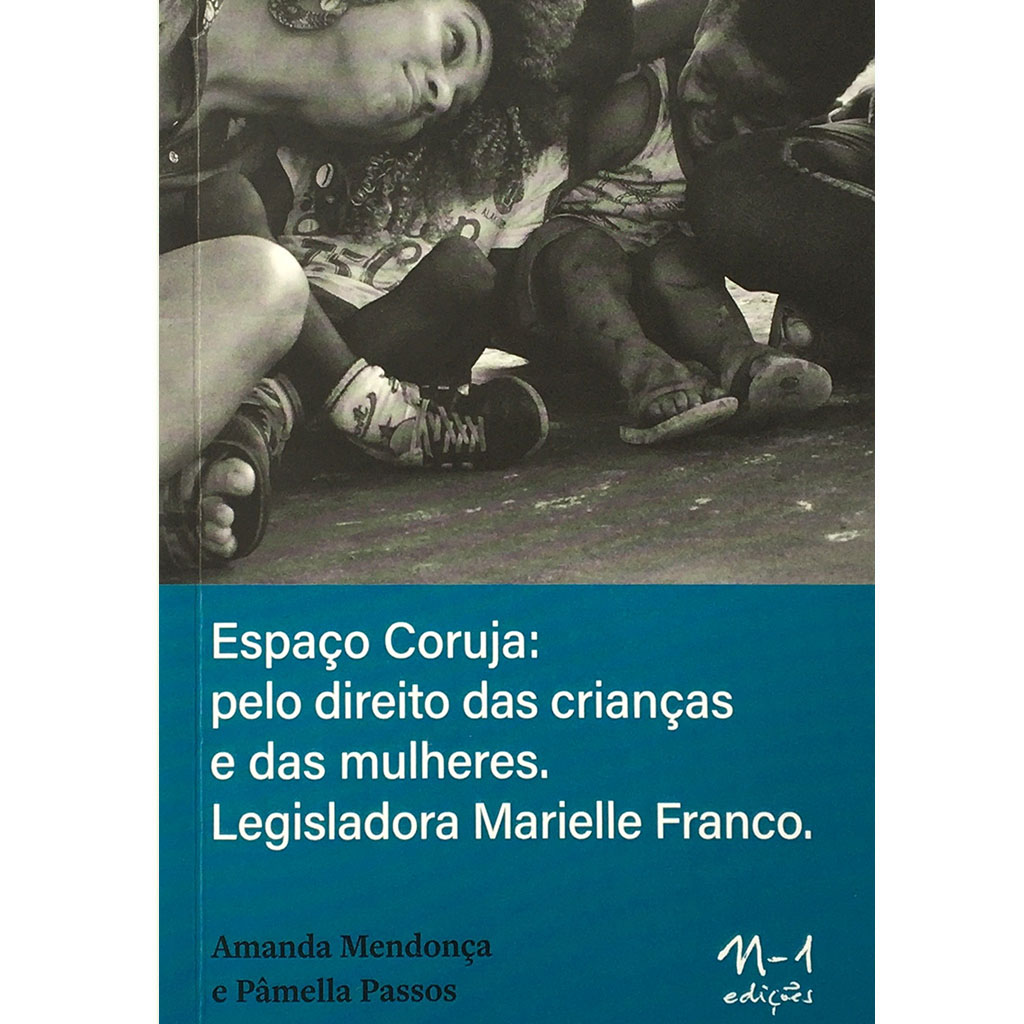
\includegraphics[width=68.5mm]{./grid/coruja.jpg}
\end{center}

\hspace*{-7cm}\hrulefill\hspace*{-7cm}

\medskip

\noindent{}A formulação do Projeto de Lei do Espaço Coruja foi uma das ações de maior impacto emocional para Marielle Franco. Era a sua história: mulher negra, que foi mãe jovem e precisava de um lugar seguro para deixar sua filha enquanto trabalhava e estudava. Com sua empatia diante da realidade dessas mulheres, propôs, como legisladora, a criação do Espaço Infantil Noturno, que, como legado, segue construindo um mundo mais justo e igualitário.

\vfill

\hspace*{-.4cm}\begin{minipage}[c]{1\linewidth}
\small{
{\Formular{\textbf{
\hspace*{-.1cm}Título: Espaço Coruja\\
Autor: Amanda Mendonça e Pâmella Passos\\ 
Editora: n-1\\
Páginas: 64\\
Formato: 10x16cm\\
Preço: R\$ 20,00\\
ISBN: 978-65-8109-705-9
}}}}
\end{minipage}

\pagebreak

\hspace{.5cm}

\begin{center}
\hspace*{-2.7cm}\raisebox{5cm}{\rotatebox[origin=t]{90}{\Formular{\textbf{Lançamento}}}}
\hspace*{2.5cm}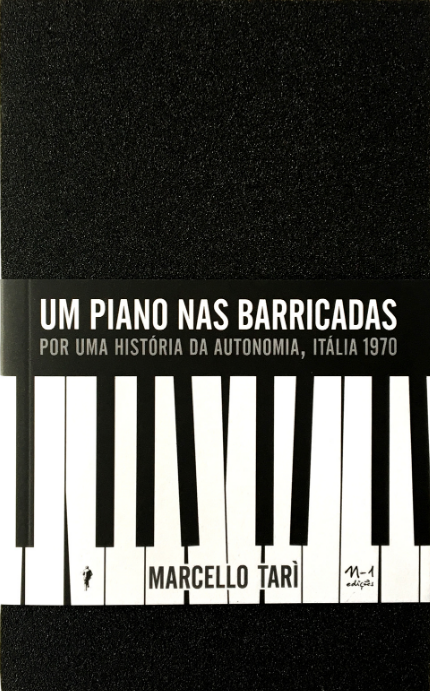
\includegraphics[width=38mm]{./imgs/barricada.png}
\end{center}

\hspace*{-7cm}\hrulefill\hspace*{-7cm}

\medskip

\noindent{}A Autonomia italiana não era uma organização, mas uma multiplicidade que se organizava a partir de onde residia, trabalhava ou estudava os sujeitos que a deram forma. Na Autonomia, de fato, muitas autonomias específicas surgiram e coexistiram: dos operários, dos estudantes, das mulheres, dos homossexuais, dos prisioneiros, melhor, de qualquer um que escolhesse, a partir de suas próprias contradições, o caminho da luta contra o trabalho assalariado e o Estado, ou seja, um modo reluzente de subversão da vida.

\vfill

\hspace*{-.4cm}\begin{minipage}[c]{1\linewidth}
\small{
{\Formular{\textbf{
\hspace*{-.1cm}Título: Um piano nas barricadas – por uma história da autonomia\\
Autor: Marcelo Tari\\ 
Editora: n-1 / Glac\\
Páginas: 384\\
Formato: 12x19cm\\
Preço: R\$ 80,00\\
ISBN: 978-65-8042-104-6 
}}}}
\end{minipage}

\pagebreak